
\section{Ajuste de la flecha} \label{sec:ajuste_flecha}

El margen de estabilidad ($\sm$ -- \emph{stability margin}) se define como la distancia entre el centro aerodinámico del ala $\left( x_\text{ac} \right)$ y el centro de gravedad $\left( x_{cg} \right)$, adimensionalizada con la cuerda media aerodinámica $\left( \mac \right)$, \ie,
\begin{equation} \label{eq:calculo_sm_1}
    \sm = X_\text{cg} = \frac{\left\lvert x_\text{cg} - x_\text{ac} \right\rvert}{\mac} 
\end{equation}
Para lograr la estabilidad en la aeronave, el centro aerodinámico debe estar detrás del centro de gravedad. Ante una perturbación en el ángulo de cabeceo de la aeronave, cuanto mayor sea $\sm$, más rápidamente volverá a la configuración original \cite{aerotools_2}. Suponiendo ala elíptica \cite{hoerner_1}, el margen de estabilidad se calcula como 
\begin{equation} \label{eq:calculo_sm_2}
    \sm = \frac{\int_0^{b/2} c(y) \, y \, dy}{\int_0^{b/2} c(y) \, d y} \tan{\Lambda} = 
    \overline{y} \tan{\Lambda}
\end{equation}
donde $\Lambda$ es la flecha del ala medida respecto de la línea de $c/4$ y $\overline{y}$ es el centroide. Variando $\Lambda$ puede lograrse el margen de estabilidad necesario. En el caso del Ho IV, este debe situarse entre $10\%$ y $15\%$.

El centroide $\overline{y}$ se puede calcular siguiendo el método geométrico propuesto por \cite{hoerner_1}. Implementando este en \MATLAB, se puede obtener el margen de estabilidad para cualquier flecha. En la figura \ref{fig:stability_margin} se representa el margen de estabilidad en función de la flecha, para $\Lambda$ en el rango $12\degrees$ a $20\degrees$.

\begin{figure}[ht]
    \centering
    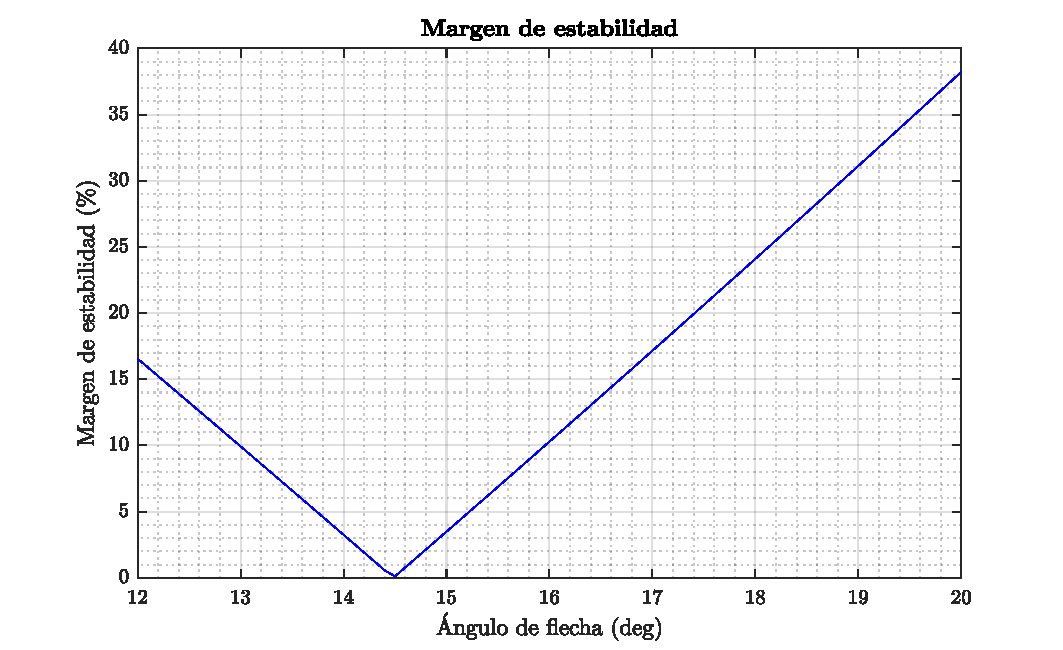
\includegraphics[width=\linewidth]{imagenes/ajuste_flecha/stability_margin.pdf}
    \caption{Margen de estabilidad $\left( \sm \right)$ en función de la flecha $\left( \Lambda \right)$ para una cuerda raíz $c_r = 1.55 \ \meter$, un estrechamiento $\lambda = 1 / 5.55$ y una envergadura $b = 20 \ \meter$.}
    \label{fig:stability_margin}
    \vspace{-4mm}
\end{figure}

Se aprecia que $\sm$ es aproximadamente lineal con $\Lambda$. Esto es debido a que puede aproximarse $\tan{\Lambda} \approx \Lambda$. Aproximadamente en $\Lambda = 14.5\degrees$, la curva no es derivable. Esto es debido al valor absoluto en \eqref{eq:calculo_sm_1}. Representando gráficamente el ala, para $\Lambda < 14.5\degrees$ el centro aerodinámico está delante del centro de gravedad. Por consiguiente es necesaria una $\Lambda > 14.5\degrees$ para lograr estabilidad estática longitudinal. Para $\Lambda$ entre $15.96\degrees$ y $16.68\degrees$ se logra el $\sm$ deseado. Como flecha definitiva se toma $\Lambda = 16.50\degrees$, con la que se logra $\sm = 13.715\%$. 


